\begin{figure}[tbh]
PRZYKLAD
\centering

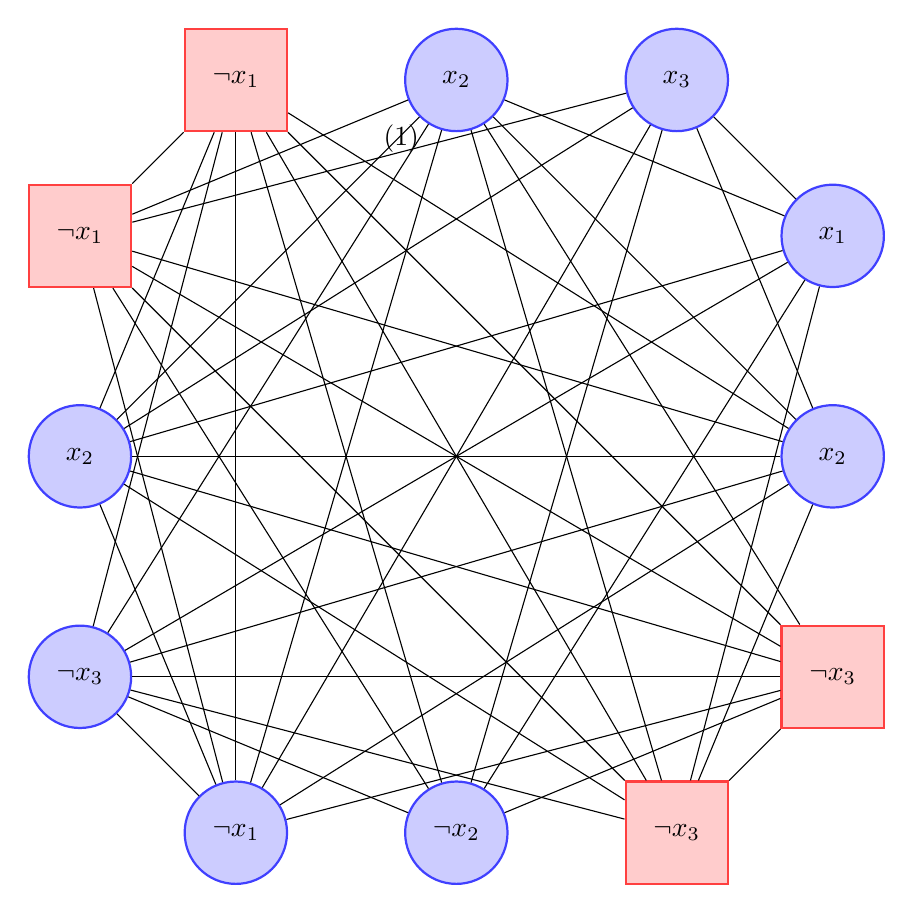
\begin{tikzpicture} [node distance=2.8cm]

\tikzstyle{unmark_vertex}=[circle,thick,draw=blue!75,fill=blue!20,minimum size=13mm]
\tikzstyle{mark_vertex}=[rectangle,thick,draw=red!75,
  			  fill=red!20,minimum size=13mm]

  \begin{scope}
  	\node [mark_vertex] (c1v1) {$\neg{x}_{1}$};
  	\node [unmark_vertex] (c1v2) [right of=c1v1] {${x}_{2}$};
  	\node [unmark_vertex] (c1v3) [right of=c1v2] {${x}_{3}$};
  	
  	\node [unmark_vertex] (c2v1) [below right of=c1v3] {${x}_{1}$}
  		edge (c1v2)
  		edge (c1v3);
  	\node [unmark_vertex] (c2v2) [below of=c2v1] {${x}_{2}$}
  		edge (c1v1)
  		edge (c1v2)
  		edge (c1v3);
  	\node [mark_vertex] (c2v3) [below of=c2v2] {$\neg{x}_{3}$}
  		edge (c1v1)
  		edge (c1v2);
  	
  	\node [mark_vertex] (c3v3) [below left of=c2v3] {$\neg{x}_{3}$}
  		edge (c1v1)
  		edge (c1v2)
  		edge (c2v1)
  		edge (c2v2)
  		edge (c2v3);
  	\node [unmark_vertex] (c3v2) [left of=c3v3] {$\neg{x}_{2}$}
  		edge (c1v1)
  		edge (c1v3)
  		edge (c2v1)
  		edge (c2v3);
  	\node [unmark_vertex] (c3v1) [left of=c3v2] {$\neg{x}_{1}$}
  		edge (c1v1)
  		edge (c1v2)
  		edge (c1v3)
  		edge (c2v2)
  		edge (c2v3);
  	
  	\node [unmark_vertex] (c4v3) [above left of=c3v1] {$\neg{x}_{3}$}
  		edge (c1v1)
  		edge (c1v2)
  		edge (c2v1)
  		edge (c2v2)
  		edge (c2v3)
  		edge (c3v1)
  		edge (c3v2)
  		edge (c3v3);
  	\node [unmark_vertex] (c4v2) [above of=c4v3] {${x}_{2}$}
  		edge (c1v1)
  		edge (c1v2)
  		edge (c1v3)
  		edge (c2v1)
  		edge (c2v2)
  		edge (c2v3)
  		edge (c3v1)
  		edge (c3v3);
  	\node [mark_vertex] (c4v1) [above of=c4v2] {$\neg{x}_{1}$}
  		edge (c1v1)
  		edge (c1v2)
  		edge (c1v3)
  		edge (c2v2)
  		edge (c2v3)
  		edge (c3v1)
  		edge (c3v2)
  		edge (c3v3);

	\node at (2.1cm, -0.75cm) {\text{(1)}};
  \end{scope}
  
  
\end{tikzpicture}

\caption{Przykład wykonania algorytmu VERTEX-COVER-EDGES-APPROX}
\label{vertex-cover-edges-approx_example}
%\small
%zakomentarzowany tekst
\end{figure}